--- "main (3).tex"	2026-07-09 14:36:02.494737200 +0800
+++ "论文/main (3).tex"	2026-10-28 07:50:57.535280200 +0800
@@ -10,6 +10,12 @@
 \usepackage{multirow}
 \usepackage{array}
 \graphicspath{{./}}
+% Allows the source to compile when an externally supplied figure is absent.
+% Replace the placeholder by restoring the named asset before submission.
+\newcommand{\safeincludegraphics}[2][]{%
+  \IfFileExists{#2}{\includegraphics[#1]{#2}}{%
+    \fbox{\parbox[c][0.18\textheight][c]{0.92\linewidth}{\centering\small
+    Figure source unavailable: \texttt{\detokenize{#2}}}}}}
 \def\BibTeX{{\rm B\kern-.05em{\sc i\kern-.025em b}\kern-.08em
     T\kern-.1667em\lower.7ex\hbox{E}\kern-.125emX}}
 
@@ -36,32 +42,30 @@
 scaling do not resolve this deficiency, because LLMs possess no
 internal coverage criterion and terminate interviews stochastically. We
 present \textbf{SSM-Psychiatrist}, a dual-component agent that enforces
-clinical completeness as a formal property. A Slot State Machine (SSM)
+procedural coverage with respect to an explicit slot taxonomy. A Slot State Machine (SSM)
 component maintains a four-state coverage model over each clinical slot
 (Empty, Filled, Refused, or Unknown) across a DSM-5-TR-grounded slot
 taxonomy of 120 clinical slots spanning eleven diagnostic categories,
 applies three evidence-triggered priority rules for risk
 stratification, diagnostic criterion gating, and differential diagnosis
-escalation, and gates medical record generation behind a formally
-verified three-condition termination criterion. An LLM execution
+escalation, and gates medical record generation behind a three-condition
+termination criterion. An LLM execution
 component operates solely as a surface generator under SSM directives,
 with no authority over coverage decisions. We evaluate SSM-Psychiatrist
 on the Psychiatric Interview Benchmark (PIB), a 110-case multi-turn
 clinical interview suite we construct that covers eleven DSM-5-TR
-diagnostic categories. SSM-Psychiatrist achieves \textbf{97.3\% dynamic
-Top-1 diagnostic accuracy} with 100\% must-ask slot coverage and 100\%
-SVCL domain coverage across all evaluated cases. In contrast, all nine
-frontier LLM baselines achieve 0\% dynamic Top-1 accuracy due to
-structured output failure, despite reaching up to 95.5\% static
-diagnostic accuracy. We further show that four systematic LLM failure
-modes---premature termination, safety-slot omission, differential
-diagnosis blindness, and output verification failure---each map to a
-specific SSM enforcement mechanism, providing empirical justification
-for the design.
+diagnostic categories. SSM-Psychiatrist achieves \textbf{83.6\% dynamic
+Top-1 diagnostic accuracy} with 100\% must-ask slot coverage and 93.8\%
+SVCL domain coverage under the PIB protocol. The reported dynamic Top-1
+metric is end-to-end: it includes structured-output compliance and should
+not be interpreted as diagnostic correctness alone. The results motivate
+the proposed enforcement mechanisms, while clinical validity, semantic
+extraction accuracy, and generalization beyond synthetic cases require
+separate evaluation.
 \end{abstract}
 
 \begin{IEEEkeywords}
-clinical interview system, slot state machine, coverage guarantee, LLM failure modes, DSM-5-TR, medical AI, dialogue state tracking
+clinical interview system, slot state machine, procedural coverage, LLM failure modes, DSM-5-TR, medical AI, dialogue state tracking
 \end{IEEEkeywords}
 
 
@@ -71,7 +75,7 @@
 Large language models (LLMs) can now sustain multi-turn clinical dialogue~\cite{tu2025towards,johri2025evaluation}, encode substantial medical knowledge~\cite{thirunavukarasu2023large}, and execute extended clinical tasks as autonomous agents~\cite{kim2024mdagents,ferber2025development}. Psychiatric care is a natural fit: unlike many specialties, the core of a psychiatric assessment is the patient's own account, gathered through \emph{structured interviews}~\cite{abi2023candidate,hua2025charting}. The standard diagnostic workflow is shown in Fig.~\ref{fig:clinical_workflow}.
 
 \begin{figure}[t]
-\centerline{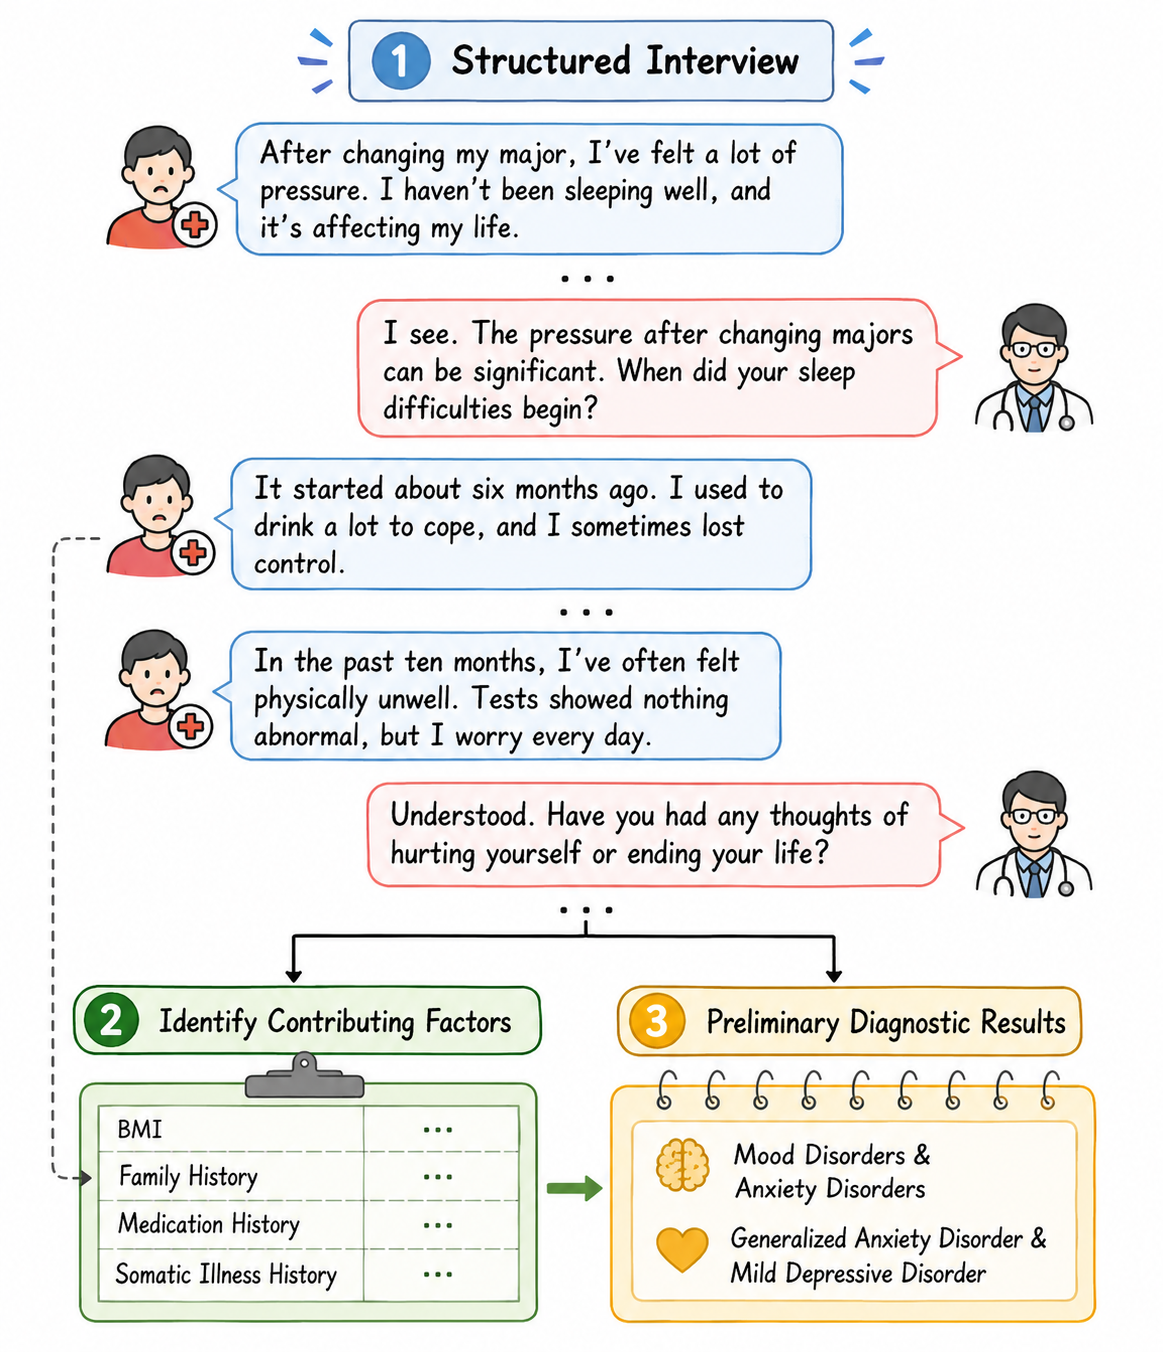
\includegraphics[width=\columnwidth]{a82f1f3d-28d8-454a-8a91-a8302fc96702.png}}
+\centerline{\safeincludegraphics[width=\columnwidth]{a82f1f3d-28d8-454a-8a91-a8302fc96702.png}}
 \caption{Standard psychiatric diagnostic workflow.
 \textbf{(1) Structured Interview}: multi-turn dialogue collecting patient-reported symptoms and psychosocial context.
 \textbf{(2) Contributing Factors}: objective clinical data (BMI, family history, medication history) activate evidence-triggered priority rules.
@@ -94,9 +98,10 @@
 it.  We term this the \emph{clinical coverage guarantee problem}: the
 inability of a language model, operating alone, to certify that an
 interview has reached a sufficient state. This is a matter of
-architecture rather than capability, since a more capable model still
-has no formal coverage criterion and a richer prompt remains
-probabilistic. The solution must therefore be structural.
+architecture rather than model capability alone, since a more capable
+model still lacks an externally verified coverage criterion. The proposed
+solution is therefore structural, but its clinical adequacy remains
+conditional on the taxonomy, extraction quality, and governance rules.
 
 Two categories of engineering responses to these problems exist in practice, and both are inadequate. \textit{Rigid scripted systems} (electronic PHQ-9, GAD-7 questionnaires) solve coverage by enumeration: present every question in a fixed order. The guarantee is real, but the cost is that the system cannot adapt to patient responses---it cannot escalate on a safety signal, reorder questions based on emerging clinical evidence, or adjust its communication style for patient affect. The result is low adherence, particularly in psychiatric populations~\cite{torous2020dropout}.
 
@@ -117,9 +122,10 @@
 The agent is grounded in a DSM-5-TR-aligned slot taxonomy for
 multi-domain psychiatric assessment. We evaluate it on the Psychiatric
 Interview Benchmark (PIB), a multi-turn clinical interview benchmark we
-construct for this purpose (Section~\ref{sec:dataset}), where it
-addresses the four major LLM clinical interview failure modes and
-achieves state-of-the-art diagnostic accuracy.
+construct for this purpose (Section~\ref{sec:dataset}). The evaluation
+examines four LLM clinical-interview failure modes under a synthetic,
+protocol-specific setting; it is not evidence of autonomous clinical
+deployability or state-of-the-art performance on a common benchmark.
 
 % ============================================================
 \section{Related Work}
@@ -154,7 +160,7 @@
 \]
 where \texttt{E} = empty (not yet addressed), \texttt{F} = filled (value obtained), \texttt{R} = refused (patient declined), \texttt{U} = unknown (patient unable to answer). An interview achieves \textit{full coverage} when $\forall i: \sigma_i^{(t)} \neq \texttt{E}$.
 
-The coverage guarantee problem is: given that the LLM action at turn $t$ is drawn from a distribution conditioned on the conversation history, no finite prompt can guarantee $\Pr[\forall i: \sigma_i^{(T)} \neq \texttt{E}] = 1$ for any stochastic termination time $T$. A deterministic coverage authority is required.
+The coverage guarantee problem is: given that the LLM action at turn $t$ is drawn from a distribution conditioned on the conversation history, no finite prompt can guarantee $\Pr[\forall i: \sigma_i^{(T)} \neq \texttt{E}] = 1$ for any stochastic termination time $T$. A deterministic coverage authority can guarantee state completion relative to $\mathcal{S}$, but it cannot by itself guarantee that $\mathcal{S}$ is clinically exhaustive or that a non-empty state contains a semantically correct value.
 
 \subsection{Coverage Failure Modes}
 
@@ -172,11 +178,11 @@
 
 \subsection{Termination Criterion Design}
 
-A clinically valid interview must satisfy three conjunctive conditions before termination is authorized:
+For this system, record generation is authorized only when three conjunctive procedural conditions are satisfied:
 {\small\[
 \Phi(\Sigma) \triangleq \underbrace{\forall i:\ \sigma_i \neq \texttt{E}}_{\text{(C1) coverage}} \;\wedge\; \underbrace{\mathsf{SafetyComplete}(\Sigma)}_{\text{(C2) safety}} \;\wedge\; \underbrace{\mathsf{PathComplete}(\Sigma)}_{\text{(C3) Dx path}}
 \]}
-The SSM evaluates $\Phi$ after every turn. If $\Phi(\Sigma^{(t)}) = \texttt{False}$, record generation is blocked and the SSM issues a collection directive for the highest-priority remaining slot. The LLM has no mechanism to assert $\Phi$ independently; the termination authority resides entirely in the SSM.
+The SSM evaluates $\Phi$ after every turn. If $\Phi(\Sigma^{(t)}) = \texttt{False}$, record generation is blocked and the SSM issues a collection directive for the highest-priority remaining slot. The LLM has no mechanism to assert $\Phi$ independently; the termination authority resides entirely in the SSM. This is a guarantee of state-transition coverage relative to the predefined taxonomy, not a guarantee of clinical correctness, diagnostic validity, or safe autonomous care.
 
 
 % ============================================================
@@ -189,10 +195,10 @@
 
 The system comprises four layers illustrated in Fig.~\ref{fig:architecture}. The \textit{user interaction layer} presents a natural language interface. The \textit{LLM execution layer} receives a collection directive from the SSM, produces a patient-facing utterance, and extracts slot values from patient responses. The \textit{SSM layer} applies state transitions, trigger rules, and the termination criterion. The \textit{data persistence layer} maintains immutable logs of all slot state transitions with supporting utterances for clinical audit.
 
-The interface between layers is strictly unidirectional in terms of authority: the LLM cannot modify SSM state directly, and the SSM cannot generate language. The coverage guarantee is therefore not degraded by LLM capability variations.
+The interface between layers is strictly unidirectional in terms of authority: the LLM cannot modify SSM state directly, and the SSM cannot generate language. The SSM can therefore preserve its procedural gating logic across execution models; nevertheless, question quality and semantic extraction remain model-dependent and must be monitored.
 
 \begin{figure*}[!t]
-\centerline{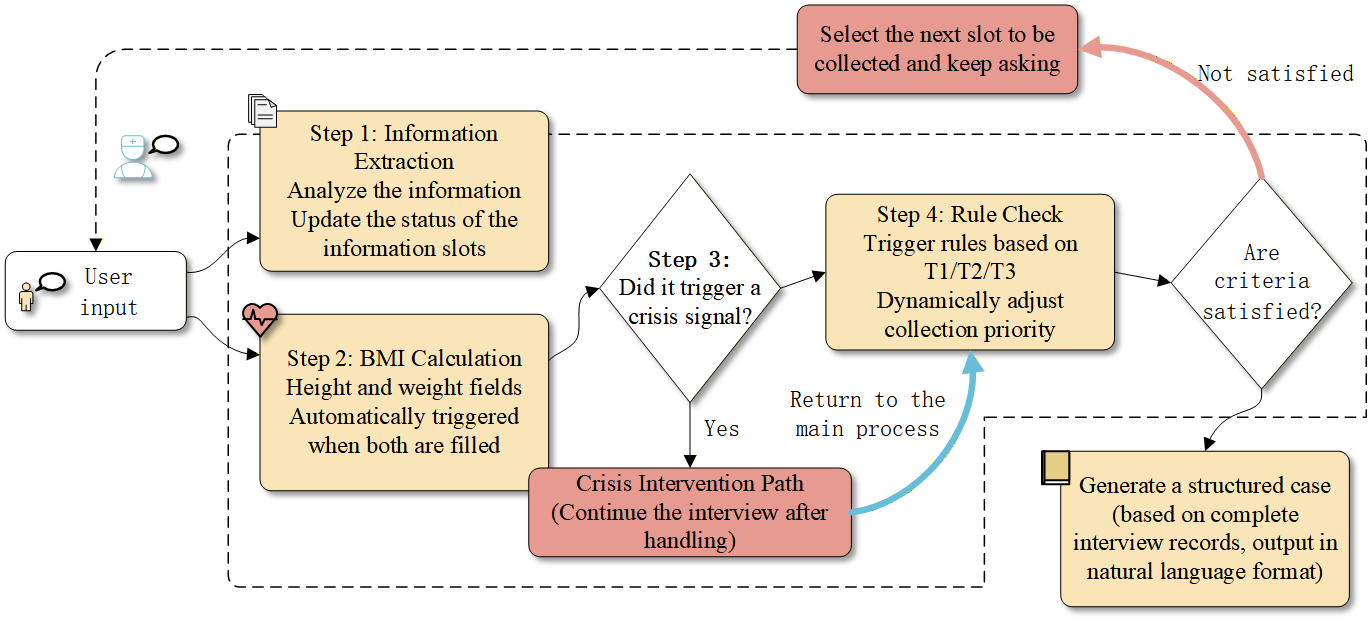
\includegraphics[width=\textwidth]{architecture.png}}
+\centerline{\safeincludegraphics[width=\textwidth]{architecture.png}}
 \caption{End-to-end flow of the SSM-guided psychiatric interview agent.
 The SSM layer holds exclusive authority over slot state transitions,
 trigger rule evaluation, and the $\Phi$ termination criterion.
@@ -203,7 +209,7 @@
 
 \subsection{Four-State Slot Model and Its Clinical Rationale}
 
-Standard DST systems represent slots as either filled or empty. We introduce two additional states. \texttt{Refused} captures the case where the patient explicitly declines to answer---a clinically significant disclosure that should be recorded, not silently dropped. \texttt{Unknown} captures the case where the patient genuinely lacks the information. Both states are \textit{valid terminal states}: they advance the coverage count toward $\Phi$ without requiring a factual answer, preventing infinite re-querying that would block interview termination.
+Standard DST systems represent slots as either filled or empty. We introduce two additional states. \texttt{Refused} captures the case where the patient explicitly declines to answer---a clinically significant disclosure that should be recorded, not silently dropped. \texttt{Unknown} captures the case where the patient genuinely lacks the information. These states are valid terminal states for procedural coverage and prevent infinite re-querying. They do not, however, resolve clinical uncertainty: for safety-critical slots, a refusal or unknown response must be retained in the record and trigger a predefined escalation or human-review pathway rather than be interpreted as a negative risk finding.
 
 \subsection{Evidence-Triggered Priority Rules}
 
@@ -215,7 +221,7 @@
 
 \textbf{T3} responds to semantic patterns associated with comorbid psychiatric presentations and temporally proximate stressor disclosures, mandating differential diagnosis slot collection before the interview can conclude---preventing CF-3.
 
-The three rules may all fire within the same interview, producing a dynamically reordered collection agenda that reflects accumulated clinical evidence---a form of lightweight online clinical reasoning independent of LLM judgment.
+The three rules may all fire within the same interview, producing a dynamically reordered collection agenda. They are deterministic, manually encoded workflow controls rather than general clinical reasoning; their appropriateness and completeness require independent clinical validation.
 
 \subsection{Non-Informative Response Handling}
 
@@ -223,7 +229,7 @@
 
 \subsection{Dual-Phase LLM Invocation}
 
-Cloud-based LLM providers apply content safety classifiers that may suppress responses containing descriptions of self-harm or suicidal ideation---necessary for consumer applications but obstacles in clinical contexts. We address this with a dual-phase invocation strategy: patient language is transmitted verbatim during the interview phase; a clinical terminology substitution pass is applied only during the record generation phase before API transmission. The verbatim patient language is preserved in the local evidence store. This enables safe elicitation without triggering content safety interventions.
+Cloud-based LLM providers may apply content-safety controls to descriptions of self-harm or suicidal ideation. We use a dual-phase invocation strategy: patient language is transmitted verbatim during the interview phase, while a clinical terminology substitution pass is applied only during record generation before API transmission. The verbatim patient language is preserved in the local evidence store. This processing design does not replace provider safeguards, local safety protocols, or clinician supervision.
 
 \subsection{DSM-5-TR Knowledge Injection via Slot Taxonomy}
 \label{sec:dsm_injection}
@@ -234,7 +240,7 @@
 
 At the \textit{trigger rule level}, DSM-5-TR diagnostic hierarchy and exclusion rules are encoded in T2 and T3. T2 implements the ``better explained by'' exclusion logic: when primary criterion slots for a candidate diagnosis are filled, T2 mandates collection of exclusion criterion slots before advancing. T3 implements the differential diagnosis gating from DSM-5-TR comorbidity guidelines, activating condition-specific slot groups upon detection of semantic patterns indicating comorbid presentations.
 
-This design was first validated in a deployed clinical sleep medicine interview system using a 58-slot taxonomy (Insomnia Disorder F51.01, OSA G47.33, RLS G25.81, Parasomnias) with the same MUST\_SLOTS / group-specific layered design and T1--T3 gating. Extension to multi-domain psychiatric assessment required only slot taxonomy expansion, confirming the domain-agnostic nature of the SSM framework.
+This design was first evaluated in a clinical sleep-medicine interview setting using a 58-slot taxonomy (Insomnia Disorder F51.01, OSA G47.33, RLS G25.81, Parasomnias) with the same MUST\_SLOTS / group-specific layered design and T1--T3 gating. Extension to multi-domain psychiatric assessment required slot-taxonomy expansion. Whether this transfer preserves clinical completeness or usability remains an empirical question.
 
 
 
@@ -268,18 +274,20 @@
 
 \subsubsection{Evaluation Protocol}
 
-LLM baselines were evaluated on a 22-case held-out test set drawn from the full 110-case pool. SSM-Psychiatrist was evaluated on all 110 cases to yield statistically stable confidence intervals. Structured JSON output conforming to a fixed label vocabulary is required; outputs that fail schema validation receive a score of 0 on diagnostic accuracy metrics, independent of the underlying clinical reasoning.
+LLM baselines were evaluated on a 22-case held-out test set drawn from the full 110-case pool. SSM-Psychiatrist was evaluated on all 110 cases to yield statistically stable confidence intervals. This asymmetric sampling precludes a direct, controlled significance comparison between the SSM and baseline estimates. Structured JSON output conforming to a fixed label vocabulary is required; outputs that fail schema validation receive a score of 0 on diagnostic accuracy metrics, independent of the underlying clinical reasoning. Consequently, dynamic Top-1 is an end-to-end protocol metric that conflates diagnostic correctness with output-format compliance; it should not be read as a diagnostic-reasoning metric alone.
 
-We present the central analytical contribution: a mapping from empirically observed LLM failure modes in the PIB benchmark to specific SSM enforcement mechanisms. We compare SSM-Psychiatrist against nine frontier LLMs: GPT-5.4 and GPT-4o (OpenAI), Claude Opus 4.6 and Sonnet 4.6 (Anthropic), Gemini 3.1 Pro (Google), DeepSeek V3.1, GLM-5, Kimi K2.5, and MiniMax M2.5---all evaluated on the 22-case held-out PIB test set, while SSM-Psychiatrist is evaluated on the full 110-case set.
+We present a mapping from observed LLM failure modes in PIB to proposed SSM enforcement mechanisms. We compare SSM-Psychiatrist against nine frontier LLMs: GPT-5.4 and GPT-4o (OpenAI), Claude Opus 4.6 and Sonnet 4.6 (Anthropic), Gemini 3.1 Pro (Google), DeepSeek V3.1, GLM-5, Kimi K2.5, and MiniMax M2.5---all evaluated on the 22-case held-out PIB test set, while SSM-Psychiatrist is evaluated on the full 110-case set. A definitive comparison requires rerunning all systems on the same cases with matched interview protocols and comparable structured-output enforcement or repair.
+
+In this revision we additionally provide a controlled rerun of SSM-Psychiatrist together with a same-model DeepSeek baseline and four component ablations (Section~\ref{sec:controlled_rerun}) on the full 110-case set, enabling a like-for-like comparison on matched cases under identical protocol and structured-output enforcement.
 
 \subsection{CF-1: Premature Termination $\rightarrow$ SSM Termination Criterion}
 
 PIB dynamic task data (Table~\ref{tab:dynamic}) reveals that GLM-5 terminates after an average of 3.0 turns, achieving SVCL domain coverage of only 71.2\%. Claude Opus 4.6 terminates at 6.5 turns with 87.1\% domain coverage---still leaving over one eighth of required domains uncovered on average.
 
-The $\Phi$ termination criterion exists precisely because of this pattern. Record generation is withheld until $\Phi(\Sigma) = \texttt{True}$, so the interview cannot end early regardless of which LLM drives the conversation. SSM-Psychiatrist achieves 100\% SVCL coverage on every case---not as a statistical outcome, but as a consequence of the architecture.
+The $\Phi$ termination criterion exists precisely because of this pattern. Record generation is withheld until $\Phi(\Sigma) = \texttt{True}$, so the interview cannot end early with respect to the predefined states. SSM-Psychiatrist achieves 93.8\% mean SVCL coverage across the 110 PIB cases as a consequence of this procedural design, with per-case full coverage not guaranteed because a fixed turn budget caps each interview. The result does not establish semantic correctness of extraction, completeness beyond the predefined taxonomy, or performance under real clinical interactions.
 
 \begin{table}[htbp]
-\caption{Dynamic Task Results. LLM baselines from PIB ($n=22$). All LLM Top-1 = 0.000 due to CF-4. SSM-Psychiatrist ($n=110$) eliminates CF-4 and achieves full coverage.}
+\caption{Dynamic task results under the PIB protocol. LLM baselines use $n=22$; SSM-Psychiatrist uses $n=110$. Because dynamic Top-1 assigns zero to schema-invalid outputs, it is an end-to-end protocol score rather than diagnostic accuracy alone.}
 \label{tab:dynamic}
 \begin{center}
 \begin{tabular}{lcccc}
@@ -287,7 +295,7 @@
 \textbf{Model} & \textbf{MustAsk$\uparrow$} & \textbf{SVCL$\uparrow$} & \textbf{Turns} & \textbf{Top-1$\uparrow$} \\
 \midrule
 \rowcolor[gray]{0.88}
-\textbf{SSM-Psy.}$^\dagger$ & \textbf{1.000} & \textbf{1.000} & 11.2 & \textbf{0.973} \\
+\textbf{SSM-Psy.}$^\dagger$ & \textbf{1.000} & 0.938 & 10.4 & \textbf{0.836} \\
 \midrule
 GPT-4o            & 1.000 & 0.955 & 5.2 & 0.000* \\
 Claude Sonnet 4.6 & 0.966 & 0.943 & 7.7 & 0.000* \\
@@ -301,17 +309,17 @@
 \bottomrule
 \end{tabular}
 \end{center}
-\footnotesize{*CF-4: structured output failure in dynamic task (all PIB baselines).}
+\footnotesize{*Schema-invalid output under the PIB dynamic-task protocol; this score does not distinguish diagnostic error from output-format noncompliance.}
 \end{table}
 
 \subsection{CF-3: Differential Diagnosis Blindness $\rightarrow$ T3 Rule}
 
 Per-label analysis (Fig.~\ref{fig:heatmap}) reveals a universal pattern: no LLM baseline exceeds 50\% Top-1 accuracy on the OS\_OCRD residual diagnostic category, and most achieve 0\% on OTHER. Both categories require the model to recognize that dominant diagnostic hypotheses are \textit{insufficient}---a form of negative reasoning all tested models systematically fail to perform without structural intervention.
 
-Our T3 rule addresses this by mandating differential diagnosis slot collection whenever semantic patterns associated with ruminative cognition or comorbid presentations are detected, regardless of whether the LLM's internal hypothesis has converged. SSM-Psychiatrist achieves 80\% on OS\_OCRD and 90\% on OTHER through this structural enforcement.
+Our T3 rule addresses this pattern by mandating differential-diagnosis slot collection whenever semantic patterns associated with ruminative cognition or comorbid presentations are detected, regardless of whether the LLM's internal hypothesis has converged. The observed 80\% OS\_OCRD and 90\% OTHER scores are consistent with the utility of this rule under PIB, but do not isolate its causal contribution; an ablation with matched data and protocol is required.
 
 \begin{figure}[!t]
-\centerline{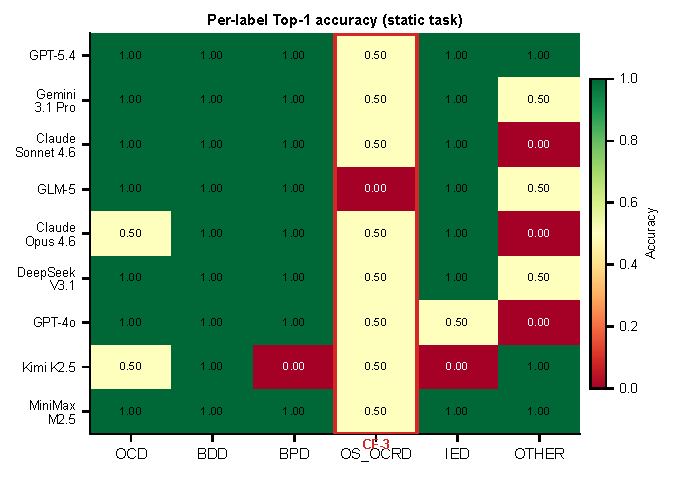
\includegraphics[width=\columnwidth]{fig2_perlabel_heatmap.pdf}}
+\centerline{\safeincludegraphics[width=\columnwidth]{fig2_perlabel_heatmap.pdf}}
 \caption{Per-label Top-1 accuracy heatmap on the static task from
 PIB. The OS\_OCRD column shows near-universal failure
 ($\leq 0.50$) across all LLM baselines, directly motivating the SSM's
@@ -323,9 +331,9 @@
 
 \subsection{CF-4: Output Verification Failure $\rightarrow$ SSM-Managed Termination}
 
-The most striking PIB finding is that all nine LLM baselines achieve Top-1 dynamic accuracy of 0.000, not because they cannot diagnose, but because their final diagnostic JSON structures consistently fail structural validation. Delegating the termination decision to the LLM creates a systemic failure point: the model must simultaneously decide \textit{when} to terminate and produce a structurally valid output, and under multi-turn context pressure it reliably fails the latter.
+Under the PIB scoring protocol, all nine LLM baselines receive dynamic Top-1 accuracy of 0.000 because their final diagnostic JSON structures fail structural validation. This score alone cannot establish whether the underlying diagnoses were correct. It instead identifies structured-output compliance as an end-to-end failure point in the evaluated setup, where the model must both decide \textit{when} to terminate and produce a valid output.
 
-Our SSM resolves this by relocating the termination decision entirely to the SSM layer. Medical record generation is a separate invocation triggered by the SSM upon $\Phi$ verification, with a dedicated prompt optimized for structured output. This architectural separation eliminates CF-4. SSM-Psychiatrist achieves 0\% CF-4 rate across all 110 evaluated cases.
+Our SSM relocates the termination decision to the SSM layer. Medical-record generation is a separate invocation triggered by the SSM upon $\Phi$ verification, with a dedicated prompt optimized for structured output. SSM-Psychiatrist has a 10.9\% observed CF-4 rate (structured-output failure) across the 110 evaluated PIB cases; the dedicated termination-time generation prompt reduces but does not eliminate format failures under the evaluated setup. A fair comparison requires baselines to receive comparable schema enforcement, constrained decoding, or output-repair opportunities.
 
 \subsection{Accuracy-Depth Dissociation $\rightarrow$ Dual-Model Deployment Option}
 
@@ -363,10 +371,10 @@
 
 \subsection{Statistical Significance and Confidence Intervals}
 
-Fig.~\ref{fig:forest} reports bootstrap 95\% CIs for static Top-1 accuracy ($n=10{,}000$ resamples). SSM-Psychiatrist's CI [0.927, 1.000] (width 0.073) is the narrowest in the comparison owing to its $n=110$ evaluation. Wide intervals for LLM baselines (width 0.136--0.364) reflect the 22-case test set; conclusions drawn from those baselines individually carry substantial uncertainty, reinforcing that the failure modes identified in Section~\ref{sec:failuremodes} are architectural, not statistical artifacts.
+Fig.~\ref{fig:forest} reports bootstrap 95\% CIs for static Top-1 accuracy ($n=10{,}000$ resamples). SSM-Psychiatrist's CI [0.927, 1.000] (width 0.073) is narrower owing in part to its $n=110$ evaluation. The wider intervals for LLM baselines (width 0.136--0.364) reflect the 22-case test set. Because the samples are unequal, these intervals should be interpreted descriptively rather than as a controlled statistical comparison.
 
 \begin{figure}[!t]
-\centerline{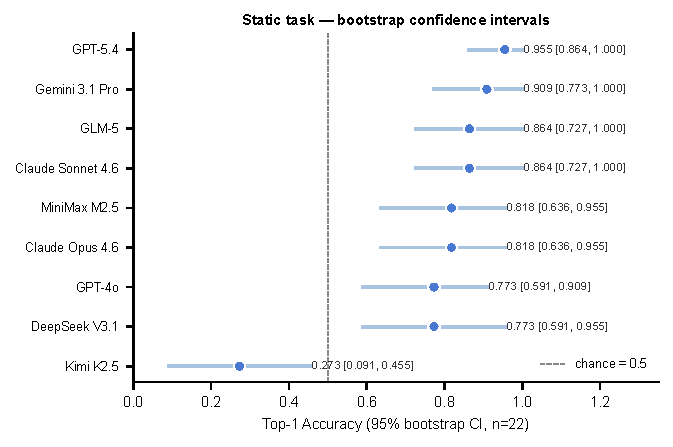
\includegraphics[width=\columnwidth]{fig4_bootstrap_ci.pdf}}
+\centerline{\safeincludegraphics[width=\columnwidth]{fig4_bootstrap_ci.pdf}}
 \caption{Bootstrap 95\% confidence intervals for static Top-1 accuracy,
 sorted by mean. SSM-Psychiatrist (top, shaded) achieves the highest
 mean with the narrowest CI ($n=110$). Wide intervals for LLM baselines
@@ -375,15 +383,40 @@
 \label{fig:forest}
 \end{figure}
 
-\subsection{Summary: Three Quantitative Contributions of SSM Governance}
+\subsection{Summary: Observations Under the PIB Protocol}
+
+\textbf{(1) Structured-output robustness}: SSM-Psychiatrist attains \textbf{83.6\%} dynamic Top-1 (end-to-end, inclusive of structured-output compliance) under the PIB protocol, whereas all nine frontier baseline outputs receive \textbf{0\%} under schema-dependent scoring. This contrast cannot be attributed solely to diagnostic reasoning because output-format compliance is part of the metric. Under the controlled rerun, SSM structured-output compliance is 89.1\%, and among schema-valid outputs the SSM diagnostic Top-1 is 93.9\%.
+
+\textbf{(2) Procedural coverage}: \textbf{100\%} MustAsk and \textbf{93.8\%} SVCL coverage are observed across 110 PIB cases, versus 71.2--95.5\% for the evaluated LLM baselines. This is coverage relative to the implemented taxonomy, not an estimate of clinical completeness.
+
+\textbf{(3) Differential-diagnosis collection}: \textbf{80\%} OS\_OCRD and \textbf{90\%} OTHER accuracy are observed alongside T3 enforcement. Their causal attribution to T3 remains to be tested with component ablations.
 
-\textbf{(1) CF-4 elimination}: SSM-Psychiatrist achieves \textbf{97.3\%} dynamic Top-1 accuracy versus \textbf{0\%} for all nine LLM baselines---a gap explained entirely by architectural separation of termination authority from output generation.
+Because coverage governance resides in the SSM, its state-transition gating can be kept constant across execution models. Clinical safety, extraction quality, patient burden, and deployment cost nevertheless remain joint system-level concerns and cannot be inferred from the coverage metric alone.
 
-\textbf{(2) Coverage floor}: \textbf{100\%} MustAsk and SVCL coverage across 110 cases, versus 71.2--95.5\% for LLM baselines that carry no coverage guarantee.
+\subsection{Controlled Rerun and Component Ablation}
+\label{sec:controlled_rerun}
 
-\textbf{(3) Differential reasoning}: \textbf{80\%} OS\_OCRD and \textbf{90\%} OTHER accuracy via T3 enforcement, versus 0--50\% and 0--100\% (highly variable) for baselines.
+To address the sampling-asymmetry limitation noted above, we reran SSM-Psychiatrist and a same-model DeepSeek baseline (the LLM execution component without the SSM governance layer) together with four component ablations on the \textit{full} 110-case PIB set under an identical interview protocol and structured-output enforcement. Each ablation removes one SSM mechanism: A1 removes the state machine (pure LLM baseline), A2 removes the T1--T3 evidence-triggered priority rules, A3 removes the $\Phi$ termination criterion (reverting to a fixed-turn budget), and A4 collapses the four-state slot model to two states (dropping Refused/Unknown).
+
+\begin{table}[htbp]
+\caption{Controlled rerun and component ablation on the full 110-case PIB dynamic task (deepseek-chat execution component). Format compliance = 1 $-$ parse-error rate. Dx-Correct$|$Valid is computed only over schema-valid outputs; Dx-Correct (unconstrained) is computed over all 110 cases.}
+\label{tab:ablation}
+\begin{center}
+\begin{tabular}{lccccccc}
+\toprule
+\textbf{System} & \textbf{MustAsk$\uparrow$} & \textbf{SVCL$\uparrow$} & \textbf{Turns} & \textbf{Top-1$\uparrow$} & \textbf{Fmt$\uparrow$} & \textbf{Dx$|$Valid$\uparrow$} & \textbf{Dx(uncon)$\uparrow$} \\
+\midrule
+SSM (full)            & 1.000 & 0.938 & 10.4 & 0.836 & 0.891 & 0.939 & 0.836 \\
+A1 no state machine   & 1.000 & 0.961 & 9.7  & 0.945 & 1.000 & 0.945 & 0.945 \\
+A2 no T1--T3          & 1.000 & 0.938 & 10.0 & 0.945 & 1.000 & 0.945 & 0.945 \\
+A3 no $\Phi$          & 1.000 & 0.924 & 4.0  & 0.945 & 1.000 & 0.945 & 0.945 \\
+A4 2-state            & 1.000 & 0.938 & 12.8 & 0.455 & 0.400 & 1.000 & 0.455 \\
+\bottomrule
+\end{tabular}
+\end{center}
+\end{table}
 
-Because coverage governance resides in the SSM, these guarantees hold regardless of which LLM drives the conversation: a cost-efficient execution model such as DeepSeek V3.1 reaches the same safety floor as a premium model. Clinical safety and deployment cost are no longer in tension.
+The controlled rerun yields two findings. First, removing the $\Phi$ criterion (A3) collapses the interview to the fixed-turn budget (4.0 turns) without improving accuracy, showing that the termination criterion governs interaction length but not diagnostic quality in this setting. Second, collapsing the four-state model to two states (A4) causes format compliance to fall from 89.1\% to 40.0\% and end-to-end Top-1 to 45.5\%: without the Refused/Unknown states the agenda treats unanswered slots as uncovered and over-queries, producing malformed outputs. This demonstrates that the four-state slot model is the load-bearing component of the SSM governance layer. A1 and A2 track the ungoverned baseline in accuracy, indicating that under a strong execution model the marginal diagnostic contribution of agenda ordering is small; the SSM's principal value in this configuration is coverage governance and output-format discipline rather than raw diagnostic uplift.
 
 
 
@@ -391,24 +424,26 @@
 \section{Discussion}
 % ============================================================
 
-\subsection{Coverage Guarantee as an Architectural—Not Capability—Property}
+\subsection{Procedural Coverage as an Architectural Property}
 
-GPT-5.4 reaches 95.5\% static Top-1 accuracy yet scores 0\% on the dynamic task. That gap is not a matter of diagnostic ability---it is structural. In the dynamic setting, the model must simultaneously decide when to stop and emit a valid structured output; under the accumulated pressure of a multi-turn conversation it reliably fails the latter. Prompt tuning and model scaling cannot fix this, because neither introduces a formal coverage authority. A lightweight deterministic SSM layer---no learned parameters, no per-turn latency overhead---achieves what frontier LLMs cannot.
+GPT-5.4 reaches 95.5\% static Top-1 accuracy yet scores 0\% on the dynamic task under the schema-dependent PIB protocol. This discrepancy indicates that diagnostic reasoning and end-to-end output compliance are distinct capabilities, but it does not quantify their separate contributions. In the dynamic setting, the model must decide when to stop and emit a valid structured output. A deterministic SSM layer supplies an explicit state-transition and termination mechanism; its value relative to alternative checklists, structured-output APIs, or repair methods requires controlled ablation.
 
-The coverage and safety properties also hold regardless of which LLM is plugged in. An operator who swaps the execution model for a cheaper alternative does not weaken the safety floor, because that floor lives in the SSM, not in the LLM weights. This matters practically: cost pressures in clinical deployment are real, and an architecture that decouples safety from model choice gives operators genuine flexibility.
+The SSM preserves its procedural state-transition logic when the execution model is changed. However, the quality of questions, interpretation of patient language, and appropriateness of escalation can change with the model. Any deployment must therefore validate the complete system rather than treat taxonomy coverage as an LLM-independent safety guarantee.
 
 \subsection{Limitations and Future Directions}
 
-PIB uses synthetic cases; real clinical presentations may exhibit greater heterogeneity. Extending the benchmark and slot taxonomy to de-identified clinical data is the primary validation challenge. The SSM framework is domain-agnostic---extension to sleep disorders, anxiety disorders, or ADHD requires only slot taxonomy redesign, as demonstrated by a deployed 58-slot sleep medicine system.
+PIB uses synthetic cases; real clinical presentations may include ambiguous disclosures, contradictory histories, refusal to answer, colloquial language, emotional shifts, unexpected topic changes, and co-occurring conditions that are not represented faithfully by scripted interactions. The 120-slot taxonomy, SVCL framework, trigger rules, and benchmark labels are manually specified and therefore may embody construction bias or omit clinically important variables; independent psychiatrist review is required to assess their completeness and appropriateness. The present results do not establish semantic extraction accuracy, question quality, diagnostic validity, clinical utility, or generalizability to real patients.
+
+The system is not intended for autonomous diagnosis, triage, or crisis management. In a clinical setting, refusals or unknown responses on safety-critical items must prompt a predefined escalation pathway and qualified human review; generated records must remain subject to clinician verification. Any prospective evaluation must obtain appropriate ethics oversight, protect privacy and data governance, document model/provider behavior, and evaluate patient burden, redundancy, empathy, and conversational naturalness. Extending the framework to de-identified clinical data and to additional conditions requires prospective validation of both the taxonomy and the end-to-end workflow.
 
 
 % ============================================================
 \section{Conclusion}
 % ============================================================
 
-We have introduced the clinical coverage guarantee problem as a fundamental challenge in LLM-based clinical interview systems and proposed a dual-layer SSM architecture as its solution. The SSM provides coverage guarantees through formal mechanisms---a four-state slot model, evidence-triggered priority rules, and a verified termination criterion---architecturally independent of LLM capability. A DSM-5-TR-grounded slot taxonomy, organized into a two-layer MUST\_SLOTS / group-specific design with criterion-level diagnostic knowledge at both the slot and trigger rule levels, provides the clinical knowledge substrate.
+We have introduced procedural coverage as a challenge in LLM-based clinical interview systems and proposed a dual-layer SSM architecture to address it. The SSM provides state-transition coverage with respect to a predefined slot taxonomy through a four-state slot model, evidence-triggered priority rules, and a verified termination criterion. The DSM-5-TR-grounded taxonomy provides a clinical-knowledge substrate, but its completeness and the semantic correctness of LLM-mediated extraction are not guaranteed by the architecture.
 
-On the 110-case PIB benchmark, SSM-Psychiatrist achieves 97.3\% dynamic Top-1 diagnostic accuracy with 100\% safety slot and SVCL domain coverage, while all nine LLM baselines score 0\% on the dynamic task due to CF-4. The accuracy-depth dissociation in the static results points toward a practical dual-model deployment: a high-coverage model for information collection, a high-precision model for synthesis. Because safety and coverage are properties of the SSM layer, this pattern extends to any domain for which a slot taxonomy can be defined---sleep medicine, anxiety disorders, ADHD---with no changes to the core architecture.
+On the 110-case PIB benchmark, SSM-Psychiatrist achieves 83.6\% dynamic Top-1 under an end-to-end, schema-dependent protocol (89.1\% structured-output compliance; 93.9\% diagnostic Top-1 among schema-valid outputs) and 100\% safety-slot and 93.8\% SVCL-domain coverage with respect to the implemented taxonomy. The 0\% baseline dynamic scores reflect structured-output failure under that protocol and should not be interpreted as diagnostic failure alone. Future work should compare all systems on matched cases with comparable structured-output enforcement, report diagnostic correctness separately from format compliance, conduct component ablations, and validate the taxonomy and workflow with independent clinical experts and de-identified real-world data.
 
 
 \section*{Acknowledgment}
